\documentclass{article}

% if you need to pass options to natbib, use, e.g.:
%     \PassOptionsToPackage{numbers, compress}{natbib}
% before loading neurips_2026

% The authors should use one of these tracks.
% Before accepting by the NeurIPS conference, select one of the options below.
% 0. "default" for submission
%\usepackage{neurips_2026}
% the "default" option is equal to the "main" option, which is used for the Main Track with double-blind reviewing.
% 1. "main" option is used for the Main Track
%  \usepackage[main]{neurips_2026}
% 2. "position" option is used for the Position Paper Track
%  \usepackage[position]{neurips_2026}
% 3. "eandd" option is used for the Evaluations & Datasets Track
 % \usepackage[eandd]{neurips_2026}
% 4. "creativeai" option is used for the Creative AI Track
%  \usepackage[creativeai]{neurips_2026}
% 5. "sglblindworkshop" option is used for the Workshop with single-blind reviewing
 % \usepackage[sglblindworkshop]{neurips_2026}
% 6. "dblblindworkshop" option is used for the Workshop with double-blind reviewing
%  \usepackage[dblblindworkshop]{neurips_2026}
% 7. "education" option is used for the Education Track
%  \usepackage[education]{neurips_2026}


% After being accepted, the authors should add "final" behind the track to compile a camera-ready version.
% 1. Main Track
 % \usepackage[main, final]{neurips_2026}
% 2. Position Paper Track
%  \usepackage[position, final]{neurips_2026}
% 3. Evaluations & Datasets Track
 % \usepackage[eandd, final]{neurips_2026}
% 4. Creative AI Track
%  \usepackage[creativeai, final]{neurips_2026}
% 5. Workshop with single-blind reviewing
  \usepackage[sglblindworkshop, final]{neurips_2026}
% 6. Workshop with double-blind reviewing
%  \usepackage[dblblindworkshop, final]{neurips_2026}
% Note. For the workshop paper template, both \title{} and \workshoptitle{} are required, with the former indicating the paper title shown in the title and the latter indicating the workshop title displayed in the footnote.
% For workshops (5., 6.), the authors should add the name of the workshop, "\workshoptitle" command is used to set the workshop title.
% \workshoptitle{WORKSHOP TITLE}
% 7. Education Track
% \usepackage[education, final]{neurips_2026}

% "preprint" option is used for arXiv or other preprint submissions
 % \usepackage[preprint]{neurips_2026}

% to avoid loading the natbib package, add option nonatbib:
%    \usepackage[nonatbib]{neurips_2026}

\usepackage[utf8]{inputenc} % allow utf-8 input
\usepackage[T1]{fontenc}    % use 8-bit T1 fonts
\usepackage{hyperref}       % hyperlinks
\usepackage{url}            % simple URL typesetting
\usepackage{booktabs}       % professional-quality tables
\usepackage{amsfonts}       % blackboard math symbols
\usepackage{nicefrac}       % compact symbols for 1/2, etc.
\usepackage{microtype}      % microtypography
\usepackage{xcolor}         % colors
\usepackage{amsmath}
\usepackage{graphicx}
\usepackage{amsthm}

%colored text for review:
\newcommand{\debp}[1]{\textcolor{red}{(\textbf{DP:} #1)}}
\newcommand{\patr}[1]{\textcolor{brown}{(\textbf{PR:} #1)}}
\newcommand{\fc}[1]{\textcolor{purple}{(\textbf{FC:} #1)}}

% math bold for lower cases (a-z)
\newcommand{\ba}{\mathbf{a}}
\newcommand{\bb}{\mathbf{b}}
\newcommand{\bc}{\mathbf{c}}
\newcommand{\bd}{\mathbf{d}}
\newcommand{\boe}{\mathbf{e}}
\newcommand{\bof}{\mathbf{f}}
\newcommand{\bg}{\mathbf{g}}
\newcommand{\bh}{\mathbf{h}}
\newcommand{\bi}{\mathbf{i}}
\newcommand{\bj}{\mathbf{j}}
\newcommand{\bk}{\mathbf{k}}
\newcommand{\bl}{\mathbf{l}}
\newcommand{\bn}{\mathbf{n}}
\newcommand{\bo}{\mathbf{o}}
\newcommand{\bp}{\mathbf{p}}
\newcommand{\bq}{\mathbf{q}}
\newcommand{\br}{\mathbf{r}}
\newcommand{\bs}{\mathbf{s}}
\newcommand{\bt}{\mathbf{t}}
\newcommand{\bu}{\mathbf{u}}
\newcommand{\bv}{\mathbf{v}}
\newcommand{\bw}{\mathbf{w}}
\newcommand{\bx}{\mathbf{x}}
\newcommand{\by}{\mathbf{y}}
\newcommand{\bz}{\mathbf{z}}

% math bold for upper cases (A-Z)
\newcommand{\bA}{\mathbf{A}}
\newcommand{\bB}{\mathbf{B}}
\newcommand{\bC}{\mathbf{C}}
\newcommand{\bD}{\mathbf{D}}
\newcommand{\bE}{\mathbf{E}}
\newcommand{\bF}{\mathbf{F}}
\newcommand{\bH}{\mathbf{H}}
\newcommand{\bI}{\mathbf{I}}
\newcommand{\bJ}{\mathbf{J}}
\newcommand{\bK}{\mathbf{K}}
\newcommand{\bL}{\mathbf{L}}
\newcommand{\bM}{\mathbf{M}}
\newcommand{\bN}{\mathbf{N}}
\newcommand{\bO}{\mathbf{O}}
\newcommand{\bP}{\mathbf{P}}
\newcommand{\bQ}{\mathbf{Q}}
\newcommand{\bR}{\mathbf{R}}
\newcommand{\bS}{\mathbf{S}}
\newcommand{\bT}{\mathbf{T}}
\newcommand{\bU}{\mathbf{U}}
\newcommand{\bV}{\mathbf{V}}
\newcommand{\bW}{\mathbf{W}}
\newcommand{\bX}{\mathbf{X}}
\newcommand{\bY}{\mathbf{Y}}
\newcommand{\bZ}{\mathbf{Z}}

% calligraphic
\newcommand{\calA}{{\mathcal{A}}}
\newcommand{\calB}{{\mathcal{B}}}
\newcommand{\calC}{{\mathcal{C}}}
\newcommand{\calD}{{\mathcal{D}}}
\newcommand{\calE}{{\mathcal{E}}}
\newcommand{\calF}{{\mathcal{F}}}
\newcommand{\calG}{{\mathcal{G}}}
\newcommand{\calH}{{\mathcal{H}}}
\newcommand{\calI}{{\mathcal{I}}}
\newcommand{\calJ}{{\mathcal{J}}}
\newcommand{\calK}{{\mathcal{K}}}
\newcommand{\calL}{{\mathcal{L}}}
\newcommand{\calM}{{\mathcal{M}}}
\newcommand{\calN}{{\mathcal{N}}}
\newcommand{\calO}{{\mathcal{O}}}
\newcommand{\calP}{{\mathcal{P}}}
\newcommand{\calQ}{{\mathcal{Q}}}
\newcommand{\calR}{{\mathcal{R}}}
\newcommand{\calS}{{\mathcal{S}}}
\newcommand{\calT}{{\mathcal{T}}}
\newcommand{\calU}{{\mathcal{U}}}
\newcommand{\calV}{{\mathcal{V}}}
\newcommand{\calW}{{\mathcal{W}}}
\newcommand{\calX}{{\mathcal{X}}}
\newcommand{\calY}{{\mathcal{Y}}}
\newcommand{\calZ}{{\mathcal{Z}}}

\newcommand{\bbA}{\mathbb{A}}
\newcommand{\bbB}{\mathbb{B}}
\newcommand{\bbC}{\mathbb{C}}
\newcommand{\bbD}{\mathbb{D}}
\newcommand{\bbE}{\mathbb{E}}
\newcommand{\bbF}{\mathbb{F}}
\newcommand{\bbG}{\mathbb{G}}
\newcommand{\bbH}{\mathbb{H}}
\newcommand{\bbI}{\mathbb{I}}
\newcommand{\bbJ}{\mathbb{J}}
\newcommand{\bbK}{\mathbb{K}}
\newcommand{\bbL}{\mathbb{L}}
\newcommand{\bbM}{\mathbb{M}}
\newcommand{\bbN}{\mathbb{N}}
\newcommand{\bbO}{\mathbb{O}}
\newcommand{\bbP}{\mathbb{P}}
\newcommand{\bbQ}{\mathbb{Q}}
\newcommand{\bbR}{\mathbb{R}}
\newcommand{\bbS}{\mathbb{S}}
\newcommand{\bbT}{\mathbb{T}}
\newcommand{\bbU}{\mathbb{U}}
\newcommand{\bbV}{\mathbb{V}}
\newcommand{\bbW}{\mathbb{W}}
\newcommand{\bbX}{\mathbb{X}}
\newcommand{\bbY}{\mathbb{Y}}
\newcommand{\bbZ}{\mathbb{Z}}

% math bold for lower cases (Greek letters)
\newcommand{\balpha}{{\boldsymbol{\alpha}}}
\newcommand{\bbeta}{{\boldsymbol{\beta}}}
\newcommand{\bgamma}{{\boldsymbol{\gamma}}}
\newcommand{\bdelta}{{\boldsymbol{\delta}}}
\newcommand{\bepsilon}{{\boldsymbol{\epsilon}}}
\newcommand{\bvarepsilon}{{\boldsymbol{\varepsilon}}}
\newcommand{\bzeta}{{\boldsymbol{\zeta}}}
\newcommand{\boldeta}{{\boldsymbol{\eta}}}
\newcommand{\btheta}{{\boldsymbol{\theta}}}
\newcommand{\bvartheta}{{\boldsymbol{\vartheta}}}
\newcommand{\biota}{{\boldsymbol{\iota}}}
\newcommand{\bkappa}{{\boldsymbol{\kappa}}}
\newcommand{\blambda}{{\boldsymbol{\lambda}}}
\newcommand{\bmu}{{\boldsymbol{\mu}}}
\newcommand{\bnu}{{\boldsymbol{\nu}}}
\newcommand{\bxi}{{\boldsymbol{\xi}}}
\newcommand{\bpi}{{\boldsymbol{\pi}}}
\newcommand{\bvarpi}{{\boldsymbol{\varpi}}}
\newcommand{\brho}{{\boldsymbol{\rho}}}
\newcommand{\bvarrho}{{\boldsymbol{\varrho}}}
\newcommand{\bsigma}{{\boldsymbol{\sigma}}}
\newcommand{\bvarsigma}{{\boldsymbol{\varsigma}}}
\newcommand{\btau}{{\boldsymbol{\tau}}}
\newcommand{\bupsilon}{{\boldsymbol{\upsilon}}}
\newcommand{\bphi}{{\boldsymbol{\phi}}}
\newcommand{\bvarphi}{{\boldsymbol{\varphi}}}
\newcommand{\bchi}{{\boldsymbol{\chi}}}
\newcommand{\bpsi}{{\boldsymbol{\psi}}}
\newcommand{\bomega}{{\boldsymbol{\omega}}}

% math bold for upper cases (Greek Letters)
\newcommand{\bGamma}{\boldsymbol{\Gamma}}
\newcommand{\bDelta}{\boldsymbol{\Delta}}
\newcommand{\bTheta}{\boldsymbol{\Theta}}
\newcommand{\bLambda}{\boldsymbol{\Lambda}}
\newcommand{\bXi}{\boldsymbol{\Xi}}
\newcommand{\bPi}{\boldsymbol{\Pi}}
\newcommand{\bSigma}{\boldsymbol{\Sigma}}
\newcommand{\bUpsilon}{\boldsymbol{\Upsilon}}
\newcommand{\bPhi}{\boldsymbol{\Phi}}
\newcommand{\bPsi}{\boldsymbol{\Psi}}
\newcommand{\bOmega}{\boldsymbol{\Omega}}

% set of numbers
\newcommand{\Real}{{\mathbb R}}
\newcommand{\Complex}{{\mathbb C}}
\newcommand{\Natural}{{\mathbb N}}
\newcommand{\Integer}{{\mathbb Z}}



\DeclareMathOperator{\Ber}{Ber}
\DeclareMathOperator{\var}{\text{var}}
\DeclareMathOperator{\gammadist}{Gamma}
\DeclareMathOperator{\betadist}{Beta}
\DeclareMathOperator{\dirdist}{Dir}
\DeclareMathOperator{\catdist}{Cat}
\DeclareMathOperator{\expdist}{Exp}
\DeclareMathOperator{\unifdist}{Unif}
\DeclareMathOperator*{\argmax}{arg\,max}
\DeclareMathOperator*{\argmin}{arg\,min}
%\DeclareMathOperator*{\supp}{supp}


\DeclareMathOperator{\supp}{supp}
\newcommand{\R}{\mathbb{R}}
\newcommand{\E}{\mathbb{E}}
\newcommand{\Prob}{\mathbb{P}}
\newcommand{\dd}{\mathrm{d}}
\newcommand{\thetahat}{\hat{\theta}_n}
\newcommand{\thetastar}{\theta^*}
\newcommand{\one}{\boldsymbol{1}}
\newcommand{\Leb}{\mathrm{Leb}}
\newcommand{\Lap}{\mathrm{Lap}}
\newcommand{\diff}{\mathrm{d}}
\newcommand{\1}{\mathbf{1}}
\newcommand{\KL}{\text{\texttt{KL}}}


\newtheorem{theorem}{Theorem}
\newtheorem{proposition}{Proposition}
\newtheorem{example}{Example}
\newtheorem{remark}{Remark}
\newtheorem{lemma}{Lemma}
\newtheorem{assumption}{Assumption}
\newtheorem{definition}{Definition}
\newcommand{\iid}{\stackrel{\mathrm{iid}}{\sim}}

% Note. For the workshop paper template, both \title{} and \workshoptitle{} are required, with the former indicating the paper title shown in the title and the latter indicating the workshop title displayed in the footnote. 
\title{Bayes-assisted anytime-valid t-tests for
Gaussian means with unknown variance}


% The \author macro works with any number of authors. There are two commands
% used to separate the names and addresses of multiple authors: \And and \AND.
%
% Using \And between authors leaves it to LaTeX to determine where to break the
% lines. Using \AND forces a line break at that point. So, if LaTeX puts 3 of 4
% authors names on the first line, and the last on the second line, try using
% \AND instead of \And before the third author name.


% \author{%
%   Debolina~Paul\thanks{Corresponding author} \\
%   Department of Statistics, University of Oxford\\
%   24-29 St Giles, OX13LB, Oxford, UK \\
%   \texttt{debolina.paul@stats.ox.ac.uk} \\
%   % examples of more authors
%   \And
%   Patrick Rebeschini \\
%   Department of Statistics,
%   University of Oxford\\
%   24-29 St Giles, OX13LB, Oxford, UK \\
%   \texttt{patrick.rebeschini@stats.ox.ac.uk} \\
%   \AND
%   Fran\c cois Caron \\
%   Department of Statistics,
%   University of Oxford\\
%   24-29 St Giles, OX13LB, Oxford, UK \\
%   \texttt{francois.caron@stats.ox.ac.uk} \\
%   % \And
%   % Coauthor \\
%   % Affiliation \\
%   % Address \\
%   % \texttt{email} \\
%   % \And
%   % Coauthor \\
%   % Affiliation \\
%   % Address \\
%   % \texttt{email} \\
% }

\author{%
  Debolina~Paul\thanks{Corresponding author}
  \hspace{1.5cm}
  Patrick~Rebeschini
  \hspace{1.5cm}
  Fran\c{c}ois~Caron
  \\
  Department of Statistics, University of Oxford\\
  24--29 St Giles, Oxford OX1 3LB, UK\\
  \texttt{\{debolina.paul, patrick.rebeschini, francois.caron\}@stats.ox.ac.uk}
}



\begin{document}


\maketitle


\begin{abstract}
  We propose an anytime-valid test of $H_0:\mu=0$ versus $H_1:\mu\neq 0$ for i.i.d.\ normal data with unknown mean $\mu$ and unknown variance $\sigma^2$, using prior information on the standardized effect size $\theta^\star=\mu/\sigma$. The test mixes a scale-invariant likelihood ratio over a prior on the effect size and applies the extended Ville inequality to obtain a valid $p$-process under arbitrary stopping. When the prior is well specified, the method improves power for alternatives favoured by the prior. For every fixed $n$ and dataset, if the prior has polynomial tails, we show that if the prior centre is moved arbitrarily far from the data, then the $p$-variable converges to a non-informative $p$-variable. Thus the procedure gains power when the prior is accurate and reverts to the non-informative benchmark under extreme prior-data conflict.
\end{abstract}



\section{Introduction}\label{sec:intro}
Student's \(t\)-test is one of the most widely used tools for testing whether a Gaussian mean is zero when the variance is unknown. Its usual validity guarantee, however, assumes a fixed sample size. In modern sequential settings, where data are monitored as they arrive or sampling stops adaptively, repeated use of fixed-sample \(p\)-values can then inflate the
Type I error rate. This motivates anytime-valid analogues of the one-sample \(t\)-test, whose evidence may be monitored continuously without invalidating inference. At the same time, many scientific problems come with genuine prior information about plausible effect sizes, which can substantially improve power, especially in sequential analyses where early rejection is valuable.


Anytime-valid testing and inference for a Gaussian mean with unknown variance has a substantial history. Most directly, \citet{Lai1976} constructed a confidence sequence for the mean, whose inversion yields an anytime-valid analogue of the one-sample $t$-test. More recent work has revisited the problem using safe testing, group invariance, and e-processes. In particular, \citet{Grunwald2024} showed that some standard Bayesian $t$-test Bayes factors \citep{Jeffreys1961,Zellner1980,Rouder2009,Gronau2020}, that incorporate prior information about the standardized effect size, are anytime valid; \citet{PerezOrtiz2024} developed a general invariant likelihood-ratio construction for anytime-valid tests with nuisance parameters; and \citet{Wang2025} gave explicit anytime-valid $t$-tests and confidence sequences. These methods establish anytime validity, but do not address how the resulting tests behave when the prior information is misspecified. Anytime validity is a property under the null and holds for any mixing measure $\Pi$, irrespective of whether it assigns mass to the effect supported by the data. Power, however, depends on the resulting mixture $M_n=\int_{\R}L_{n,\theta} \, \Pi(\dd\theta)$. As the prior centre moves away from the true standardised effect, this mixture can become arbitrarily small. Whether this loss of evidence translates into a loss of power depends on the calibration used to convert $M_n$ into a $p$-process.  

We study this issue in the Gaussian model $Y_1,Y_2,\ldots \stackrel{\mathrm{iid}}{\sim}\mathcal N(\mu,\sigma^2)$, with $\theta^\star=\mu/\sigma$ as the standardised effect-size, where both $\mu$ and $\sigma>0$ are unknown, to test $H_0:\theta^\star=0$ against $H_1:\theta^\star\neq0$. Our objective is to construct an anytime-valid $p$-process $(P_n)_{n\geq2}$ satisfying $\sup_{\sigma>0}\Prob_{0,\sigma}(\inf_{n\geq2}P_n\leq\alpha)\leq\alpha$
for $\alpha\in(0,1)$, that exploits informative prior information when it is accurate while remaining useful under severe misspecification. Following the literature above, we mix the scale-invariant likelihood ratio $L_{n,\theta}$ over a prior $\Pi$, $M_n=\int_\R L_{n,\theta}\,\Pi(\dd\theta)$. For a proper prior, $M_n$ is a test martingale. The standard reciprocal Ville calibration $P_n^V=\min\{1,1/M_n\}$ \citep{Ville1939,Shafer2011,Ramdas2023} preserves anytime validity, but can be highly sensitive to prior misspecification. When the prior moves away from the true effect, the mixture martingale $M_n$ can tend to $0$ and $P_n^V$ to one, eliminating power even though validity is retained. We therefore consider the extended Ville calibration of \citet{Wang2025a}. Starting at $n_0=2$, let us define
$g(c)=\sup_{\sigma>0}\E_{0,\sigma}[\min\{1,M_2/c\}]$ for $c>0$, and set $P_n^E=g(M_n)$. This calibration is also  anytime-valid and for a proper prior satisfies $g(c)\leq\min\{1,1/c\}$, so it is pointwise no more conservative than reciprocal Ville calibration. 

Our contributions are twofold. First, we identify a generic failure of reciprocal Ville calibration under prior misspecification. For any proper location prior, fixed sample size, and dataset with positive sample variance, the test martingale \(M_{n}\) converges to zero as the prior centre \(m\) is moved arbitrarily far from the true effect size. Consequently, \(P_{n}^{V}\) tends to $1$, irrespective of how strongly the data contradict the null. The test remains anytime-valid for every prior centre \(m\), but its fixed-horizon power vanishes under extreme prior misspecification. Second, we %show that extended Ville calibration provides a robust fallback. If the proper location prior has polynomial tails, then, for every fixed sample size and every dataset with positive sample variance, the extended-Ville-calibrated $p$-value converges, under extreme prior--data conflict, to the non-informative anytime-valid $t$-test of \citet{Lai1976}, preserving a nondegenerate benchmark where reciprocal calibration degenerates to one. Calibration, rather than anytime-validity itself, is therefore the decisive ingredient in robustness to prior misspecification. %This extends the bounded-influence, extended-Ville programme of \citet{Cortinovis2025} to the classical unknown-variance $t$-testing problem, and is reminiscent of work in the Bayesian literature on bounded-influence priors \citep{Dawid1973,Pericchi1992,Pericchi1995}.
extend the bounded-influence, extended-Ville framework of \citet{Cortinovis2025} from the known-variance Gaussian mean problem to the unknown-variance $t$-testing setting. After eliminating the nuisance parameter $\sigma$ by invariance, the Gaussian likelihood becomes $L_{n,\theta}=e^{-n\theta^2/2}A_n(\theta U_n)$, where $A_n$ is the moment generating function of a $\chi_n$ random variable and $U_n$ is the maximal invariant. Unlike the known-variance case, the tails of $A_n(\theta U_n)$ partially offsets the Gaussian factor, so the effective decay depends on $n-U_n^2$. A direct dominated-convergence argument therefore fails and instead we derive a two-sided integrable envelope and combine it with regular variation of the prior tails to derive the asymptotics of the translated mixture. A further complication is that the Lebesgue mixture is infinite at $n=1$ and finite only from $n_0=2$, so extended-Ville calibration must begin at $U_2$. We therefore prove both $\frac{M_{n,m}}{a_m}\longrightarrow M_n^{\mathrm{Leb}}$ and $g_m(a_m c)\longrightarrow g_{\mathrm{Leb}}(c)$, where $a_m = \pi(-m)$. The common factor $a_m$ cancels upon composition, yielding $g_m(M_{n,m})\longrightarrow g_{\mathrm{Leb}}(M_n^{\mathrm{Leb}})$ and recovering the non-informative test of \citet{Lai1976}. This cancellation fails under reciprocal Ville calibration, where the factor $a_m$ remains and the resulting $p$-value converges to $1$. This phenomenon connects naturally to the bounded-influence perspective in the Bayesian literature \citep{Dawid1973,Pericchi1992,Pericchi1995}.
\vspace{-4pt}
\section{Background}
\label{sec:background}
\vspace{-4pt}
\paragraph{Scale-invariant likelihood-ratio mixtures.}
The null family corresponding to $H_0:\theta^\star=0$ is
$\mathcal P_0=\{\mathcal N(0,\sigma^2):\sigma>0\}$. Following
\citet{Lai1976,PerezOrtiz2024,Wang2025}, we remove the unknown scale by
working with the filtration
$\mathcal F_n=\sigma(Y_1/|Y_1|,Y_2/|Y_1|,\ldots,Y_n/|Y_1|)$. Define
$U_n=\sum_{i=1}^nY_i/(\sum_{i=1}^nY_i^2)^{1/2}\in[-\sqrt n,\sqrt n]$ and
let $A_n(z)=\E[e^{zR_n}]$, $R_n\sim\chi_n$, be the moment generating
function of a $\chi_n$ random variable. For $\theta\in\R$, the likelihood
ratio of the reduced data under standardized effect $\theta$, relative to
standardized effect zero, is
\begin{equation}
\label{eq:hthetadef}
  L_{n,\theta}=e^{-n\theta^2/2}A_n(\theta U_n).
\end{equation}
For each fixed $\theta$, $(L_{n,\theta})_{n\geq1}$ is an
$(\mathcal F_n)$-test martingale under every distribution in
$\mathcal P_0$; writing $T_n$ for the usual one-sample $t$-statistic,
$U_n=\sqrt n\,T_n/\{(n-1)+T_n^2\}^{1/2}$ almost surely for $n\geq2$. Let
$\Pi$ be a nonzero $\sigma$-finite measure on $\R$, representing a mixing
measure over standardized effect sizes, and set
$M_n=\int_\R L_{n,\theta}\,\Pi(\dd\theta)$. If $\Pi$ is a probability
distribution then $(M_n)_{n\geq1}$ is a test martingale; in general it is
an extended nonnegative martingale.

\paragraph{Calibration.}
We use the common starting time $n_0=2$, both for proper mixtures and for
the Lebesgue benchmark below. For a proper $\Pi$, ordinary Ville
calibration gives $P_n^V=\min\{1,1/M_n\}$, $n\geq2$. The extended Ville
calibration of \citet{Wang2025a} uses the null law of the evidence at the
starting time: define $g(0)=1$, $g(\infty)=0$ and
\begin{equation}
\label{eq:general-extended-calibration}
  g(c)=\E_{0,1}\!\left[\min\left\{1,\frac{M_2}{c}\right\}\right],
  \quad c>0,
  \qquad
  P_n^E=g(M_n),
  \quad n\geq2,
\end{equation}
the expectation being computable under any $\mathcal N(0,\sigma^2)$ since
$M_2$ is scale invariant. Whenever $M_n$ is finite a.s.
$\forall n\geq2$, $P_n^E$ is a $p$-process, even if $\Pi$ is merely
$\sigma$-finite and $M_n$ is not integrable. The running
versions are
$\widetilde P_n^V=\min\{1,1/\max_{2\leq k\leq n}M_k\}$ and
$\widetilde P_n^E=g(\max_{2\leq k\leq n}M_k)$. Extended Ville calibration is also unaffected by the normalisation of the mixing measure; multiplying $\Pi$ by $a>0$ multiplies $M_n$ by $a$ and replaces $g(c)$ by $g(c/a)$, leaving $g(M_n)$ unchanged.
\vspace{-4pt}
\paragraph{The Lebesgue benchmark.}
The improper Lebesgue mixing measure $\Pi_{\Leb}(\dd\theta)=\dd\theta$
provides the noninformative benchmark of \citet{Lai1976,Wang2025}. Here
$M_1^{\Leb}=\infty$ almost surely, whereas $M_n^{\Leb}<\infty$ almost
surely for every $n\geq2$; thus $(M_n^{\Leb})_{n\geq2}$ is a
finite-valued extended nonnegative martingale, but not an integrable test
martingale.

\begin{proposition}[Lebesgue mixture]
\label{prop:Mn-Leb}
For every $n\geq2$, on $\{|U_n|<\sqrt n\}$,
$M_n^{\Leb}=\sqrt{2\pi/n}\,(1-U_n^2/n)^{-n/2}$. Define $g_{\Leb}(0)=1$,
$g_{\Leb}(\infty)=0$ and, for $c>0$, write $q=\sqrt\pi/c$; then
\begin{equation}
\label{eq:g-Leb}
  g_{\Leb}(c)=1 \quad\text{if } q\geq1,
  \qquad
  g_{\Leb}(c)
  =\frac{2}{\pi}\left[\arcsin\!\left(\sqrt q\right)+\sqrt{q(1-q)}\right]
  \quad\text{if } q<1 .
\end{equation}
Then $P_n^{\Leb}:=g_{\Leb}(M_n^{\Leb})$ and
$\widetilde P_n^{\Leb}:=g_{\Leb}(\max_{2\leq k\leq n}M_k^{\Leb})$,
$n\geq2$, are $p$-processes for $\mathcal P_0$.
\end{proposition}



\section{Main results}
\label{sec:mainresult}
\vspace{-4pt}
\subsection{Prior-location misspecification}
\label{subsec:location-misspecification}
\vspace{-4pt}
Let $\pi$ be a probability density on $\R$, regarded as a zero-location
baseline density. Holding its shape and scale fixed, consider the
location family $\Pi_m(\dd\theta)=\pi_m(\theta)\,\dd\theta$, where
$\pi_m(\theta)=\pi(\theta-m)$ and $m\in\R$. Here $m$ is a user-specified
working-prior location, rather than an unknown parameter to be estimated,
and $|m-\theta^\star|$ measures location misspecification. We study an
extreme-misspecification path by fixing $\theta^\star$, the prior shape,
and the sample size, and then letting $m\to+\infty$ or $m\to-\infty$.
This is a prior-sensitivity limit, not a large-sample limit: the results
below hold pointwise for each fixed dataset with positive sample
variance. For $n\geq2$ and $u\in(-\sqrt n,\sqrt n)$, define
\vspace{-4pt}
\begin{equation}
\label{eq:hnu-def}
  h_n(\theta,u)=e^{-n\theta^2/2}A_n(u\theta),
  \ 
  M_{n,m}(u)=\int_\R h_n(\theta,u)\pi(\theta-m)\,\dd\theta,
  \ 
  M_n^{\Leb}(u)=\int_\R h_n(\theta,u)\,\dd\theta,
\end{equation}
so that $M_{n,m}=M_{n,m}(U_n)$, while $M_n^{\Leb}=M_n^{\Leb}(U_n)$ is the
Lebesgue-mixture benchmark of Section~\ref{sec:background}. Specializing
the calibrations to $\Pi_m$, define
$g_m(c)=\E_{0,1}[\min\{1,M_{2,m}/c\}]$ for $c>0$, with $g_m(0)=1$ and
$g_m(\infty)=0$, and set $P_{n,m}^V=\min\{1,1/M_{n,m}\}$ and
$P_{n,m}^E=g_m(M_{n,m})$, with running versions
$\widetilde P_{n,m}^V$ and $\widetilde P_{n,m}^E$ defined analogously.
Our first result does not require any tail condition on $\pi$.

\begin{proposition}[Degeneracy of reciprocal Ville calibration]
\label{prop:ville-degeneracy}
Let $\pi$ be any probability density. For every $n\geq2$ and every
$u\in(-\sqrt n,\sqrt n)$, $M_{n,m}(u)\to0$ as $m\to+\infty$ or
$m\to-\infty$. Consequently, for every fixed dataset $y_{1:n}$ with
positive sample variance, $P_{n,m}^V\to1$ as $|m|\to\infty$; and if, in
addition, every prefix $y_{1:k}$, $2\leq k\leq n$, has positive sample
variance, then $\widetilde P_{n,m}^V\to1$ as $|m|\to\infty$.
\end{proposition}

Under every nondegenerate Gaussian model, all prefix sample variances are
positive almost surely. Writing $\Prob_{\theta^\star,\sigma}$ for the law
under which $Y_i\iid\mathcal N(\sigma\theta^\star,\sigma^2)$,
Proposition~\ref{prop:ville-degeneracy} and bounded convergence imply
that $\Prob_{\theta^\star,\sigma}(P_{n,m}^V\leq\alpha)\to0$ and
$\Prob_{\theta^\star,\sigma}(\widetilde P_{n,m}^V\leq\alpha)\to0$ as
$|m-\theta^\star|\to\infty$, for every fixed $\theta^\star\in\R$,
$\sigma>0$, $n\geq2$ and $\alpha\in(0,1)$. When $\theta^\star\neq0$ both
the fixed-time power and the probability of rejection by time $n$ thus
vanish: anytime-validity is retained for every $m$, but the reciprocal
calibration becomes uninformative.
\vspace{-4pt}
\subsection{Recovery under regularly varying tails}
\label{subsec:recovery}\vspace{-4pt}
We next impose a tail condition that determines the limiting behaviour of extended Ville calibration.

\begin{assumption}[Regularly varying prior tails]
\label{ass:tails}
There exist $\beta>1$ and positive slowly varying functions $L_+$ and
$L_-$ such that, as $x\to\infty$, $\pi(x)\sim x^{-\beta}L_+(x)$ and
$\pi(-x)\sim x^{-\beta}L_-(x)$.
\end{assumption}

This condition is satisfied by Student $t$ densities with $\nu>0$ degrees
of freedom, for which $\beta=\nu+1$; the Cauchy case has $\beta=2$. For
sufficiently large $|m|$, define $a_m=\pi_m(0)=\pi(-m)$. Under
Assumption~\ref{ass:tails}, for every fixed $R<\infty$,
\vspace{-4pt}
\begin{equation}
\label{eq:prior-local-flattening}
  \sup_{|\theta|\leq R}
  \left|\frac{\pi(\theta-m)}{a_m}-1\right|\longrightarrow0
  \qquad\text{as }m\to+\infty\text{ or }m\to-\infty,
\end{equation}
so that the rescaled shifted prior is asymptotically flat on every
bounded set.

\begin{theorem}[Recovery of the Lebesgue benchmark]
\label{thm:recovery}
Fix $n\geq2$ and a dataset $y_{1:n}$ with positive sample variance, and
write
$u_n=\sum_{i=1}^ny_i/(\sum_{i=1}^ny_i^2)^{1/2}\in(-\sqrt n,\sqrt n)$.
With all evidence quantities evaluated at this fixed dataset,
Assumption~\ref{ass:tails} implies, along either $m\to+\infty$ or
$m\to-\infty$,
\begin{equation}
\label{eq:recovery-limits}
  \frac{M_{n,m}}{a_m}\longrightarrow M_n^{\Leb},
  \qquad
  g_m(a_mc)\longrightarrow g_{\Leb}(c)\ \ (c>0),
  \qquad
  P_{n,m}^E=g_m(M_{n,m})\longrightarrow P_n^{\Leb} .
\end{equation}
If every prefix $y_{1:k}$, $2\leq k\leq n$, has positive sample variance,
then also $\widetilde P_{n,m}^E\to\widetilde P_n^{\Leb}$ as
$|m|\to\infty$.
\end{theorem}

The mechanism is the local flattening in
\eqref{eq:prior-local-flattening}, the exponential envelope for $h_n$ in Lemma~\ref{lemma:hthetabound} makes the contribution from large $|\theta|$ negligible, so the mixture only sees the region on which
$\pi(\theta-m)\approx a_m$, whence $M_{n,m}\approx a_mM_n^{\Leb}$. The same argument at the calibration time $n=2$ gives $g_m(a_mc)\to g_{\Leb}(c)$, and monotonicity of $g_m$ then yields the composition limit. The vanishing factor $a_m$ is retained by reciprocal calibration but cancels in the extended Ville, which is the reason we get $P_{n,m}^V\to1$ and $P_{n,m}^E\to P_n^{\Leb}$.
\vspace{-4pt}
\section{Experiments}
\label{sec:experiments}
\vspace{-8pt}
\begin{figure}[!h]
    \centering    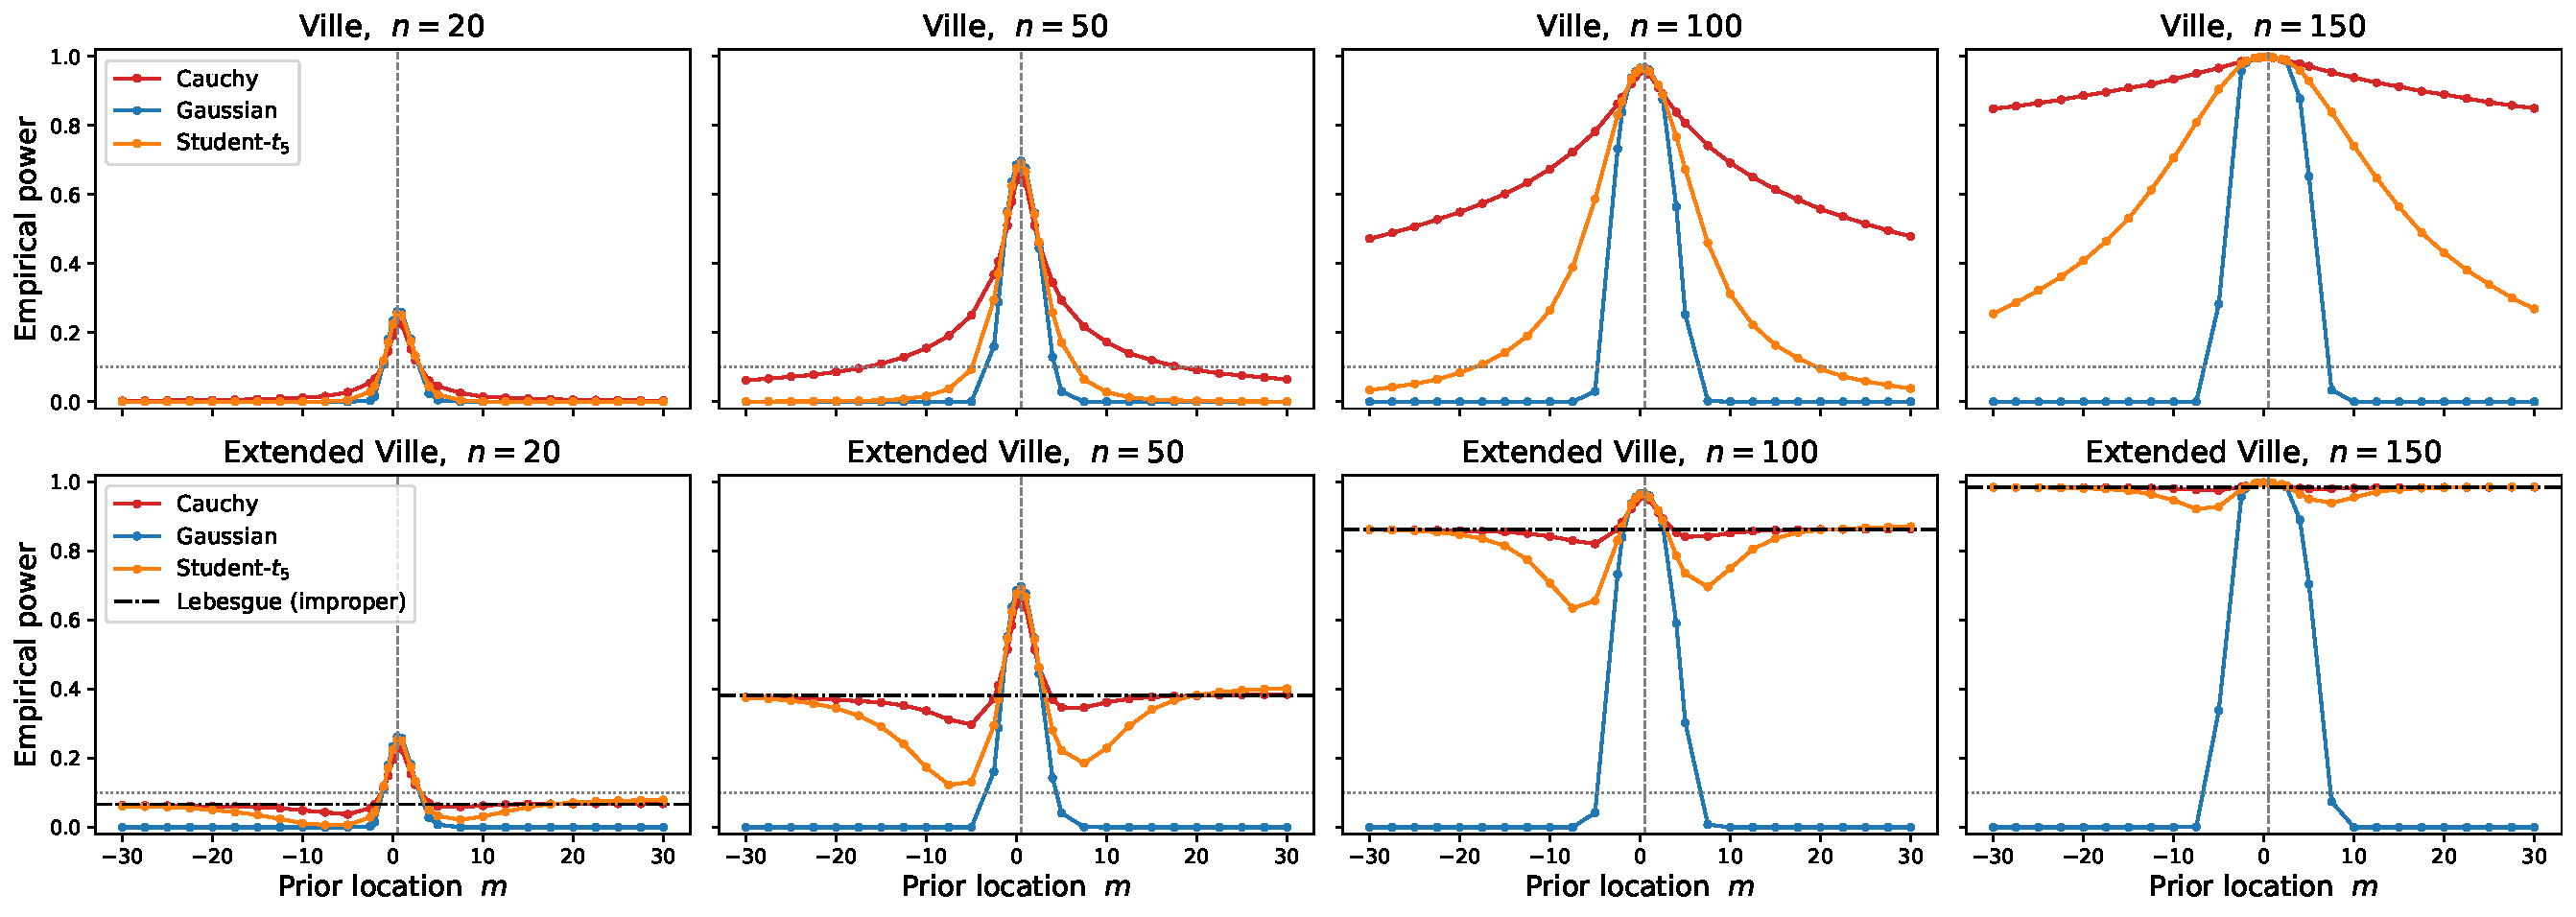
\includegraphics[width=\linewidth,height=0.32\linewidth]{images/power_vs_m_priors.pdf}
    \caption{Empirical power of the Ville (top) and extended-Ville (bottom) procedures against the prior location $m$, with $\theta^\star=0.5$, $n\in\{20,50,100,150\}$, $B=10{,}000$ data and
    $B_{\mathrm{cal}}=100{,}000$ calibration replicates. Dashed vertical line for $m=\theta^\star$, dotted line for $\alpha=0.1$, dash-dotted black line is the Lebesgue baseline.}
    \label{fig:power_vs_m}
\end{figure}
\vspace{-4pt}
\paragraph{Simulation study.}
We set $\sigma=1$, so that data generated from $\mathcal N(0.5,1)$
coincide with the standardised effect size $\theta^\star=0.5$, and test
$H_0:\theta=0$ against $H_1:\theta\neq0$ at fixed sample size
$n\in\{20,50,100,150\}$ with level $\alpha=0.1$. For each prior $\pi$ and
each location $m$ on a grid over $[-30,30]$ we draw $B=10{,}000$ datasets
$Y_{1:n}^{(b)}\iid\mathcal N(\theta^\star,1)$ and report the empirical
Ville and extended-Ville rejection rates. We compare the proper priors
Cauchy (with the Rouder--JZS default scale $1/\sqrt2\approx0.707$),
Gaussian (with $\sigma=1$) and Student-$t$ (with $5$ degrees of freedom
and unit scale); the improper Lebesgue prior serves as a non-informative
baseline in the extended Ville. The marginal likelihoods have no closed
form here and are computed by adaptive Gauss--Kronrod quadrature in
$\theta$ \citep{piessens2012quadpack}, and the calibrations $g_m$ by
Monte Carlo under $\Prob_0$ with $B_{\mathrm{cal}}=100{,}000$
replicates. Figure~\ref{fig:power_vs_m}
shows that both procedures attain their maximum power near the true
effect $\theta^\star=0.5$ and decrease as the prior--data conflict
increases. The Ville power eventually drops to $0$, while the extended
Ville reverts back to the Lebesgue baseline, making it robust against
prior--data conflict.

% \paragraph{A sequential test of a training-run specification.}
% Training the same architecture with different random seeds gives
% different held-out accuracy, and each observation costs a full
% training run, so stopping as soon as the evidence permits is valuable.
% Using Fashion-MNIST \citep{Xiao2017}, we train $N=1{,}200$
% single-hidden-layer perceptrons on subsamples of a fixed training pool
% and evaluate each on a fixed disjoint held-out set, so that the
% accuracies $A_i$ are i.i.d.\ conditional on that set; with $b$ a
% benchmark fixed in advance we set $Y_i=A_i-b$, test
% $H_0:\theta^\star=0$ two-sided at level $\alpha=0.05$, and record the
% number of networks that must be trained before rejection. The Lebesgue procedure rejects
% after $165$ runs, and at locations at or near the truth all three
% families reject after roughly $140$. As $m$ increases the families
% separate: the Gaussian prior requires $585$ runs at $m=8$ and fails to
% reject at all for $m\geq16$, exhausting the budget of $1{,}200$ runs,
% whereas the Cauchy and Student-$t_5$ priors return to the Lebesgue
% baseline at $m=32$ and $m=64$: a polynomial-tail prior asserting an effect two orders
% of magnitude beyond the truth costs nothing relative to using no prior
% information, which is the recovery of Theorem~\ref{thm:recovery} against
% the failure of the Gaussian. The
% extended-Ville first-rejection time is at or before its Ville counterpart
% everywhere, and the gap is largest under severe
% conflict: at $m=32$ with the Student-$t_5$ prior, extended Ville rejects
% after $165$ runs against $535$ for Ville, a saving of $370$ training
% runs.
\vspace{-4pt}
\section{Discussion}
\label{sec:discussion}\vspace{-4pt}
For the anytime-valid $t$-test, robustness to prior misspecification is driven more by the choice of calibration than by anytime-validity itself. Regular variation can be viewed as the zero-rate case of a broader directional limit, under which a Laplace prior still yields a non-degenerate, though directional, fallback. Two natural open questions are to establish a quantitative rate in $|m-\theta^\star|$ and to extend the analysis to prior-scale misspecification.

\bibliographystyle{plainnat}
\bibliography{robustttest}


\appendix

\section{Secondary lemma}
\label{app:lemma}

\begin{lemma}
\label{lemma:hthetabound}
For \(n\geq2\), \(|u|<\sqrt n\), and \(\theta\in\mathbb R\), let
\begin{equation}
\label{eq:hthetadef2}
  h_n(\theta,u)
  =
  e^{-n\theta^2/2}A_n(\theta u),
\end{equation}
where \(A_n\) is the moment generating function of \(\chi_n\). For any
\(\eta\) such that \(u^2<\eta<n\),
\begin{equation}
\label{eq:hu-env}
  h_n(\theta,u)
  \leq
  \exp\left\{-\frac{(n-\eta)\theta^2}{2}\right\}
  \left(1-\frac{u^2}{\eta}\right)^{-n/2}.
\end{equation}
Consequently, there exist constants \(C_{n,u},\kappa_{n,u}>0\) such
that
\[
  0\leq h_n(\theta,u)
  \leq C_{n,u}e^{-\kappa_{n,u}\theta^2}.
\]
\end{lemma}

\begin{proof}
Let \(R_n\sim\chi_n\). Young's inequality gives
\[
  u\theta R_n
  \leq
  \frac{\eta\theta^2}{2}
  +
  \frac{u^2R_n^2}{2\eta}.
\]
Therefore,
\begin{align*}
  h_n(\theta,u)
  &=
  \mathbb E\left[
    \exp\left\{-\frac{n\theta^2}{2}+u\theta R_n\right\}
  \right]
  \\
  &\leq
  \exp\left\{-\frac{(n-\eta)\theta^2}{2}\right\}
  \mathbb E\left[
    \exp\left\{\frac{u^2R_n^2}{2\eta}\right\}
  \right]
  \\
  &=
  \exp\left\{-\frac{(n-\eta)\theta^2}{2}\right\}
  \left(1-\frac{u^2}{\eta}\right)^{-n/2},
\end{align*}
because \(R_n^2\sim\chi_n^2\) and \(u^2/\eta<1\).
\end{proof}

\section{Proof of Proposition~\ref{prop:Mn-Leb}}
\label{app:proof-Leb}

\begin{proof}
For \(u\in(-\sqrt n,\sqrt n)\), Tonelli's theorem and the Gaussian
integral give
\begin{align*}
  M_n^{\Leb}(u)
  &=
  \int_{\mathbb R}
  e^{-n\theta^2/2}A_n(u\theta)\,\dd\theta
  \\
  &=
  \mathbb E\left[
    \int_{\mathbb R}
    \exp\left(-\frac{n\theta^2}{2}+u\theta R_n\right)
    \dd\theta
  \right]
  \\
  &=
  \sqrt{\frac{2\pi}{n}}
  \mathbb E\left[
    \exp\left(\frac{u^2R_n^2}{2n}\right)
  \right],
  \qquad R_n\sim\chi_n.
\end{align*}
Since \(R_n^2\sim\chi_n^2\),
\[
  \mathbb E\left[
    \exp\left(\frac{u^2R_n^2}{2n}\right)
  \right]
  =
  \left(1-\frac{u^2}{n}\right)^{-n/2},
\]
which proves the first result. The expectation diverges when
\(|u|=\sqrt n\). In particular, \(|U_1|=1\) almost surely, so
\(M_1^{\Leb}=\infty\). For \(n\geq2\), equality in
\(|U_n|\leq\sqrt n\) requires \(Y_1=\cdots=Y_n\), an event of
probability zero under every nondegenerate Gaussian model. Hence
\(M_n^{\Leb}<\infty\) almost surely for every \(n\geq2\).

It remains to compute the calibration at time two. By
using $U_n
  =
  \frac{n\widehat\theta_n}
       {\sqrt{(n-1)+n\widehat\theta_n^2}}
  =
  \frac{\sqrt n\,T_n}
       {\sqrt{(n-1)+T_n^2}}$ and $M_n^{\Leb}
  =
  \sqrt{\frac{2\pi}{n}}
  \left(1-\frac{U_n^2}{n}\right)^{-n/2}$, we get,
\[
  M_2^{\Leb}
  =
  \sqrt\pi\,(1+T_2^2),
\]
and, under the null, \(T_2\sim t_1\), the standard Cauchy
distribution. Thus \(V=\arctan(T_2)\) is uniform on
\((-\pi/2,\pi/2)\). If \(0<c\leq\sqrt\pi\), then
\(M_2^{\Leb}/c\geq1\) almost surely and \(g_{\Leb}(c)=1\). If
\(c>\sqrt\pi\), put \(q=\sqrt\pi/c\in(0,1)\) and
\(a=\arccos(\sqrt q)\). Then
\begin{align*}
  g_{\Leb}(c)
  &=
  \frac1\pi
  \int_{-\pi/2}^{\pi/2}
  \min\{1,q\sec^2 v\}\,\dd v
  \\
  &=
  \frac1\pi
  \left(
    2q\tan a+\pi-2a
  \right)
  \\
  &=
  \frac{2}{\pi}
  \left[
    \arcsin(\sqrt q)+\sqrt{q(1-q)}
  \right],
\end{align*}
which is \eqref{eq:g-Leb}. Extended Ville calibration then yields both $P_n^{\Leb}$ and its running-maximum version.
% For $u\in(-\sqrt n,\sqrt n)$, Tonelli's theorem and the Gaussian integral
% give
% \[
%   M_n^{\Leb}(u)
%   =\int_\R e^{-n\theta^2/2}A_n(u\theta)\,\dd\theta
%   =\E\left[\int_\R
%      \exp\left\{-\frac{n\theta^2}{2}+u\theta R_n\right\}\dd\theta\right]
%   =\sqrt{\frac{2\pi}{n}}\,
%    \E\!\left[e^{u^2R_n^2/(2n)}\right],
% \]
% with $R_n\sim\chi_n$. Since $R_n^2\sim\chi_n^2$, the expectation equals
% $(1-u^2/n)^{-n/2}$, which proves the stated closed form; on $\{S_n>0\}$
% it may equivalently be written as
% $\sqrt{2\pi/n}\,(1+n\widehat\theta_n^2/(n-1))^{n/2}$, where
% $\widehat\theta_n=\overline Y_n/S_n$. The expectation diverges when
% $|u|=\sqrt n$; in particular $|U_1|=1$ almost surely, so
% $M_1^{\Leb}=\infty$. For $n\geq2$, equality in $|U_n|\leq\sqrt n$
% requires $Y_1=\cdots=Y_n$, an event of probability zero under every
% nondegenerate Gaussian model, so that $M_n^{\Leb}<\infty$ almost surely.

% It remains to compute the calibration at time two. Since
% $U_2=\sqrt2\,T_2/(1+T_2^2)^{1/2}$, with $T_2$ the $t$-statistic, we have
% $M_2^{\Leb}=\sqrt\pi\,(1+T_2^2)$, and under the null $T_2\sim t_1$, the
% standard Cauchy distribution, so that $V=\arctan(T_2)$ is uniform on
% $(-\pi/2,\pi/2)$. If $0<c\leq\sqrt\pi$ then $M_2^{\Leb}/c\geq1$ almost
% surely and $g_{\Leb}(c)=1$. If $c>\sqrt\pi$, put $q=\sqrt\pi/c\in(0,1)$
% and $a=\arccos(\sqrt q)$; then
% \[
%   g_{\Leb}(c)
%   =\frac1\pi\int_{-\pi/2}^{\pi/2}\min\{1,q\sec^2v\}\,\dd v
%   =\frac{2q\tan a+\pi-2a}{\pi}
%   =\frac2\pi\left[\arcsin(\sqrt q)+\sqrt{q(1-q)}\right],
% \]
% which is \eqref{eq:g-Leb}. Extended Ville calibration then yields both
% $P_n^{\Leb}$ and its running-maximum version.
\end{proof}

\section{Proof of Proposition~\ref{prop:ville-degeneracy}}
\label{app:proof-degeneracy}

\begin{proof}
Let \(Z\) have density \(\pi\).  The change of variables
\(\theta=m+z\) gives
\[
  M_{n,m}(u)
  =
  \mathbb E\bigl[h_n(m+Z,u)\bigr].
\]
For \(\lvert u\rvert<\sqrt n\), Lemma~\ref{lemma:hthetabound} gives
constants \(C_{n,u},\kappa_{n,u}>0\) such that
\[
  0
  \leq
  h_n(\theta,u)
  \leq
  C_{n,u}e^{-\kappa_{n,u}\theta^2}
  \leq
  C_{n,u},
  \qquad \theta\in\mathbb R.
\]
For every fixed \(z\),
\(h_n(m+z,u)\to0\) as \(|m|\to\infty\).  Dominated convergence therefore proves $M_{n,m}(u)\to0$, and $P_{n,m}^V\to1$ follows. For the running version, apply the same limit to each of the finitely many prefixes $k=2,\ldots,n$; their maximum also converges to zero.

% Let $Z$ have density $\pi$. The change of variables $\theta=m+z$ gives
% $M_{n,m}(u)=\E[h_n(m+Z,u)]$. For $|u|<\sqrt n$,
% Lemma~\ref{lemma:hthetabound} gives constants $C_{n,u},\kappa_{n,u}>0$
% such that
% $0\leq h_n(\theta,u)\leq C_{n,u}e^{-\kappa_{n,u}\theta^2}\leq C_{n,u}$
% for all $\theta\in\R$. For every fixed $z$, $h_n(m+z,u)\to0$ as
% $|m|\to\infty$. Dominated convergence therefore proves
% $M_{n,m}(u)\to0$, and $P_{n,m}^V\to1$ follows. For the running version,
% apply the same limit to each of the finitely many prefixes
% $k=2,\ldots,n$; their maximum also converges to zero.
\end{proof}

\section{Proof of Theorem~\ref{thm:recovery}}
\label{app:proof-recovery}

\begin{proof}
    We recall that
$$
h_{n}(\theta,u)=e^{-n\theta^2/2 }A_n(u \theta ).
$$
Write $M_{n,m}(u)=\int_{\mathbb R} h_n(\theta,u)\pi(\theta-m)\,\dd\theta$ and $M_n^\Leb(u)=\int_{\mathbb R} h_n(\theta,u)\,\dd\theta$.

\emph{Step 1 (ratio convergence).}  Fix $R>0$ and split
\[
  \frac{M_{n,m}(u)}{a_m}
  \;=\;\underbrace{\int_{|\theta|\leq R}}_{=:I_1(R,m)}
   +\underbrace{\int_{R<|\theta|\leq m/2}}_{=:I_2(R,m)}
   +\underbrace{\int_{|\theta|>m/2}}_{=:I_3(m)}\;
   h_{n}(\theta,u)\,\frac{\pi(\theta-m)}{a_m}\,\dd\theta.
\]
We have, for any $\theta$,
$$
\pi(\theta-m)\sim a_m \sim m^{-\beta}L_-(m)
$$
as $m\to\infty$. By the uniform convergence theorem for regularly varying functions
\citep[Theorem~1.2.1]{Bingham1987},
$$
\sup_{|\theta|\leq R}|\pi(\theta-m)/a_m-1|\to 0
$$
as $m\to\infty$, so
$$
I_1(R,m)\to\int_{|\theta|\leq R}h_{n}(\theta,u)\,\dd\theta.
$$
For $I_2$, on $|\theta|\leq m/2$ we have $|\theta-m|\in[m/2,\,3m/2]$, so
regular variation yields a constant $C_\star<\infty$ (independent of $R$ and of
$m$ for all large $m$) such that $\pi(\theta-m)/a_m\leq C_\star$; hence
$$
I_2(R,m)\leq C_\star\int_{|\theta|>R}h_{n}(\theta,u)\,\dd\theta,
$$ which vanishes
as $R\to\infty$. For $I_3$, using the fact that $\pi$ is a proper prior
(i.e.\ $\int_\mathbb{R}\pi=1$),
\[
I_3(m)\;=\;\int_{|\theta|>m/2}h_{n}(\theta,u)\,\frac{\pi(\theta-m)}{a_m}\,\dd\theta
   \;\leq\; a_m^{-1}\sup_{|\theta|>m/2}h_{n}(\theta,u),
\]
the supremum is exponentially small in $m$ by \eqref{eq:hu-env}, while $a_m$ is
only polynomially small, so $I_3(m)\to 0$.

Combining these three bounds, for each fixed $R>0$,
\begin{align*}
   \int_{|\theta|\leq R}h_{n}(\theta,u)\,\dd\theta
   \;\leq\; \liminf_{m\to\infty}\frac{M_{n,m}(u)}{a_m}
   &\;\leq\; \limsup_{m\to\infty}\frac{M_{n,m}(u)}{a_m}\\
   & \;\leq\; \int_{|\theta|\leq R}h_{n}(\theta,u)\,\dd\theta
   \;+\; C_\star\!\int_{|\theta|>R}h_{n}(\theta,u)\,\dd\theta.
\end{align*}
Sending $R\to\infty$ and using $\int_\mathbb{R} h_{n}(\theta,u)\,\dd\theta
= M_n^{\Leb}(u)$ gives the first limit in
\eqref{eq:recovery-limits}.

\emph{Step 2 (calibration convergence).}
Since \(|U_2|<\sqrt 2\) almost surely under \(\Prob_0\), Step~1 applied with \(n=2\) gives
\(M_{2,m}(U_2)/a_m\to M_2^{\Leb}(U_2)\) almost surely. Since \(0\leq\min(M_{2,m}(U_2)/(a_m c),1)\leq 1\), bounded convergence yields
\[
  g_m(a_m c)
  \;=\;\E_0\!\Bigl[\min\!\Bigl(\tfrac{M_{2,m}(U_2)}{a_mc},1\Bigr)\Bigr]
  \;\longrightarrow\;
  \E_0\!\Bigl[\min\!\Bigl(\tfrac{M_2^{\Leb}(U_2)}{c},1\Bigr)\Bigr]
  \;=\;g_{\Leb}(c),
\]
which is the second limit in \eqref{eq:recovery-limits}.

\emph{Step 3 (composition).}
Set \(c_m:=M_{n,m}(u_n)/a_m\) and \(c:=M_n^{\Leb}(u_n)\); by Step~1 \(c_m\to c\). Each \(g_m\) is decreasing, so for any \(\varepsilon\in(0,c)\) and \(m\) large, \(g_m(a_m(c+\varepsilon))\leq g_m(a_m c_m)\leq g_m(a_m(c-\varepsilon))\). Taking \(\liminf\) and \(\limsup\) using Step~2 and letting \(\varepsilon\downarrow 0\) yields the third limit in \eqref{eq:recovery-limits}. The running version follows by applying Step~1 to each of the finitely many prefixes $k=2,\ldots,n$, taking the maximum, and repeating the monotonicity argument.
\end{proof}

% \begin{proof}
% Recall that $h_n(\theta,u)=e^{-n\theta^2/2}A_n(u\theta)$, and write
% $M_{n,m}(u)=\int_\R h_n(\theta,u)\pi(\theta-m)\,\dd\theta$ and
% $M_n^{\Leb}(u)=\int_\R h_n(\theta,u)\,\dd\theta$. We treat
% $m\to+\infty$; the case $m\to-\infty$ is symmetric.

% \emph{Step 1 (ratio convergence).} Fix $R>0$ and split
% \[
%   \frac{M_{n,m}(u)}{a_m}
%   =\underbrace{\int_{|\theta|\leq R}}_{=:I_1(R,m)}
%   +\underbrace{\int_{R<|\theta|\leq m/2}}_{=:I_2(R,m)}
%   +\underbrace{\int_{|\theta|>m/2}}_{=:I_3(m)}
%   h_n(\theta,u)\frac{\pi(\theta-m)}{a_m}\,\dd\theta .
% \]
% Since $\pi(\theta-m)\sim a_m\sim m^{-\beta}L_-(m)$ as $m\to\infty$, the
% uniform convergence theorem for regularly varying functions
% \citep[Theorem~1.2.1]{Bingham1987} gives
% $\sup_{|\theta|\leq R}|\pi(\theta-m)/a_m-1|\to0$, and hence
% $I_1(R,m)\to\int_{|\theta|\leq R}h_n(\theta,u)\,\dd\theta$. For $I_2$, on
% $|\theta|\leq m/2$ we have $|\theta-m|\in[m/2,3m/2]$, so regular
% variation yields a constant $C_\star<\infty$, independent of $R$ and of
% $m$ for all large $m$, such that $\pi(\theta-m)/a_m\leq C_\star$; hence
% $I_2(R,m)\leq C_\star\int_{|\theta|>R}h_n(\theta,u)\,\dd\theta$, which
% vanishes as $R\to\infty$. For $I_3$, using the fact that $\pi$ is a
% proper prior,
% $I_3(m)\leq a_m^{-1}\sup_{|\theta|>m/2}h_n(\theta,u)$; the supremum is
% exponentially small in $m$ by \eqref{eq:hbound}, while $a_m$ is only
% polynomially small, so $I_3(m)\to0$. Combining these three bounds, for
% each fixed $R>0$,
% \[
%   \int_{|\theta|\leq R}h_n\,\dd\theta
%   \leq\liminf_{m\to\infty}\frac{M_{n,m}(u)}{a_m}
%   \leq\limsup_{m\to\infty}\frac{M_{n,m}(u)}{a_m}
%   \leq\int_{|\theta|\leq R}h_n\,\dd\theta
%    +C_\star\int_{|\theta|>R}h_n\,\dd\theta ,
% \]
% where $h_n=h_n(\theta,u)$.
% Sending $R\to\infty$ and using
% $\int_\R h_n(\theta,u)\,\dd\theta=M_n^{\Leb}(u)$ gives the first limit in
% \eqref{eq:recovery-limits}.

% \emph{Step 2 (calibration convergence).} Since $|U_2|<\sqrt2$ almost
% surely under $\Prob_0$, Step~1 applied with $n=2$ gives
% $M_{2,m}(U_2)/a_m\to M_2^{\Leb}(U_2)$ almost surely. Since
% $0\leq\min\{M_{2,m}(U_2)/(a_mc),1\}\leq1$, bounded convergence yields
% \[
%   g_m(a_mc)
%   =\E_0\left[\min\left\{\frac{M_{2,m}(U_2)}{a_mc},1\right\}\right]
%   \longrightarrow
%   \E_0\left[\min\left\{\frac{M_2^{\Leb}(U_2)}{c},1\right\}\right]
%   =g_{\Leb}(c),
% \]
% which is the second limit in \eqref{eq:recovery-limits}.

% \emph{Step 3 (composition).} Set $c_m:=M_{n,m}(u_n)/a_m$ and
% $c:=M_n^{\Leb}(u_n)$; by Step~1, $c_m\to c$. Each $g_m$ is decreasing, so
% for any $\varepsilon\in(0,c)$ and $m$ large,
% $g_m(a_m(c+\varepsilon))\leq g_m(a_mc_m)\leq g_m(a_m(c-\varepsilon))$.
% Taking $\liminf$ and $\limsup$ using Step~2 and letting
% $\varepsilon\downarrow0$ yields the third limit in
% \eqref{eq:recovery-limits}. The running version follows by applying
% Step~1 to each of the finitely many prefixes $k=2,\ldots,n$, taking the
% maximum, and repeating the monotonicity argument.
% \end{proof}


\end{document}